\documentclass[12pt]{report}
\usepackage[a4paper, left=2cm, right=2cm]{geometry}
\usepackage{xcolor}
\definecolor{grey}{rgb}{0.9,0.9,0.9}
\usepackage[utf8]{inputenc}
\usepackage[T1]{fontenc}
%\usepackage[sfdefault]{ClearSans}
\usepackage[sfdefault,light]{FiraSans}
%\usepackage{XCharter} % Use the XCharter font (serif)
\usepackage{graphicx}
\renewcommand{\contentsname}{Spis treści}
\usepackage{hyperref}
\hypersetup{
	colorlinks,
	citecolor=black,
	filecolor=black,
	linkcolor=black,
	urlcolor=black
}
\renewcommand{\chaptername}{}


\begin{document}
	\begin{titlepage} 
		\begin{center}
			
\includegraphics[scale=0.4]{agh.jpg}
		\end{center}

	\vfill
		\colorbox{grey}{
			\parbox[t]{0.93\textwidth}{
				\parbox[t]{0.91\textwidth}{
					\raggedleft
					\fontsize{50pt}{80pt}\selectfont
					\vspace{0.7cm}
					CoffeeLand\\
					\fontsize{20pt}{50pt}\selectfont
					Projekt sklepu internetowego\\
					\fontsize{15pt}{30pt}\selectfont
					Inżynieria Oprogramowania\\
					\vspace{0.7cm}
					
				}
			}
		}
	
		\vfill
		\parbox[t]{0.93\textwidth}{
			\raggedleft
			\large
			{\Large Aneta Pociecha}\\[4pt]
			{\Large Magdalena Tragarz}\\[4pt]
			{\Large Marek Ochocki}\\[4pt]
			{\Large Artur Bugaj}\\[4pt]
			\hfill\rule{0.2\linewidth}{1pt}\\[12pt]
			{Prowadzący zajęcia: dr inż. Marek Zachara}\\[4pt]
		}	
	\end{titlepage}
	
	%---------------------------------------------------------
	
	\newpage
	
	\tableofcontents

	\setcounter{chapter}{0}	
	\setcounter{section}{0}	
	
	
%---------------------------------------	
	\chapter{Streszczenie działania systemu}
	
	\section{Cel systemu}
	
		\paragraph{}
		
		Celem realizowanego systemu jest stworzenie prostego w użyciu sklepu internetowego z kawą. Zakupy wymagają założenia konta. Wybór produktów odbywa się poprzez katalog znajdujący się na stronie głównej. Klikając na produkt można przejść do osobnej strony ze szczegółowymi informacjami. Dodawanie produktów do koszyka odbywa się z poziomu podstrony produktu. W koszyku klient ma możliwość złożenia zamówienia. Płatność jest realizowana poprzez system PayPal. W sklepie Coffee Land został przewidziany system reklamacji.
	
	\section{Opis funkcjonalności z punktu widzenia klienta}
		
		\subsection{Wejścia systemu}
					\begin{itemize}
						\item formularz rejstracji 
						\item formularz logowania
						\item filtracja po typie kawy i cenie
						\item wprowadzenie danych adresowych
						\item formularz reklamacji
						\item edycja danych w profilu
						\item zapis do newslettera
					\end{itemize}

	
	\subsection{Lista możliwości}
		\begin{itemize}
			\item rejstracja użytkownika
			\item logowanie użytkownika
			\item zakup produktu
			\item reklamacja
			\item filtrowanie oferty ze względu na typ produktu i zakres ceny
			\item zapis do newslettera
			\item rezygnacja z newslettera
			\item dodanie adresu do listy adresów
			\item usunięcie adresu z listy adresów
			\item edycja danych użytkownika
		\end{itemize}


	\section{Opis funkcjonalności z punktu widzenia pracownika}

	\subsection{Wejścia systemu}
		\begin{itemize}
			\item 
			\item 
			\item
		\end{itemize}
	
	
	\subsection{Lista możliwości}
	\begin{itemize}
		\item 
		\item 
		\item
	\end{itemize}
	
%---------------------------------------	
	\chapter{Diagram kontekstowy}

	\begin{center}
			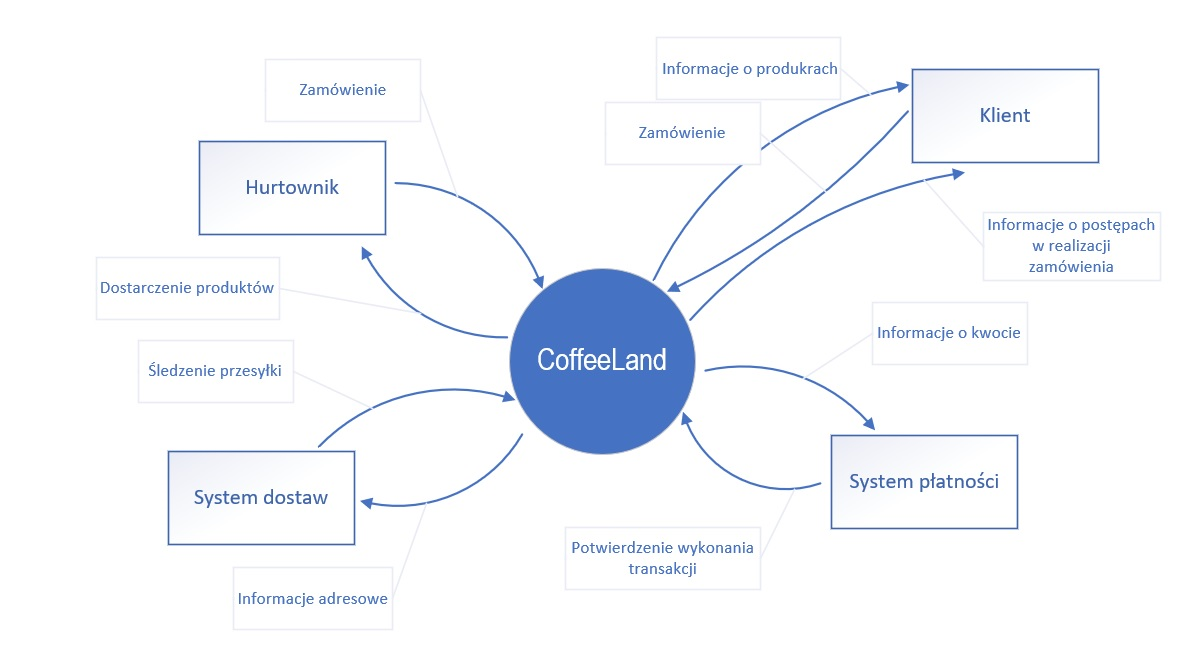
\includegraphics[scale=0.6]{kontekstowy.png}
	\end{center}
%---------------------------------------	
	%\renewcommand{\thesection}{\arabic{section}}
	
	\chapter{Funkcjonalności}
	\section{Rejstracja}
	\section{Logowanie}
	\section{Wylogowanie}
	\section{Zakup produktu}
	\section{Reklamacja}	
	\section{Filtrowanie produktów}
	\section{Zapis do newslettera}
	\section{Rezygnacja z newslettera}
	\section{Dodanie adresu do listy adresów}
	\section{Usunięcie adresu z listy adresów}
	\section{Edycja danych użytkownika}
		
	
	
%---------------------------------------	

	\renewcommand{\thesection}{\thechapter.\arabic{section}}		
	
	\chapter{Model danych - diagramy ERD}

	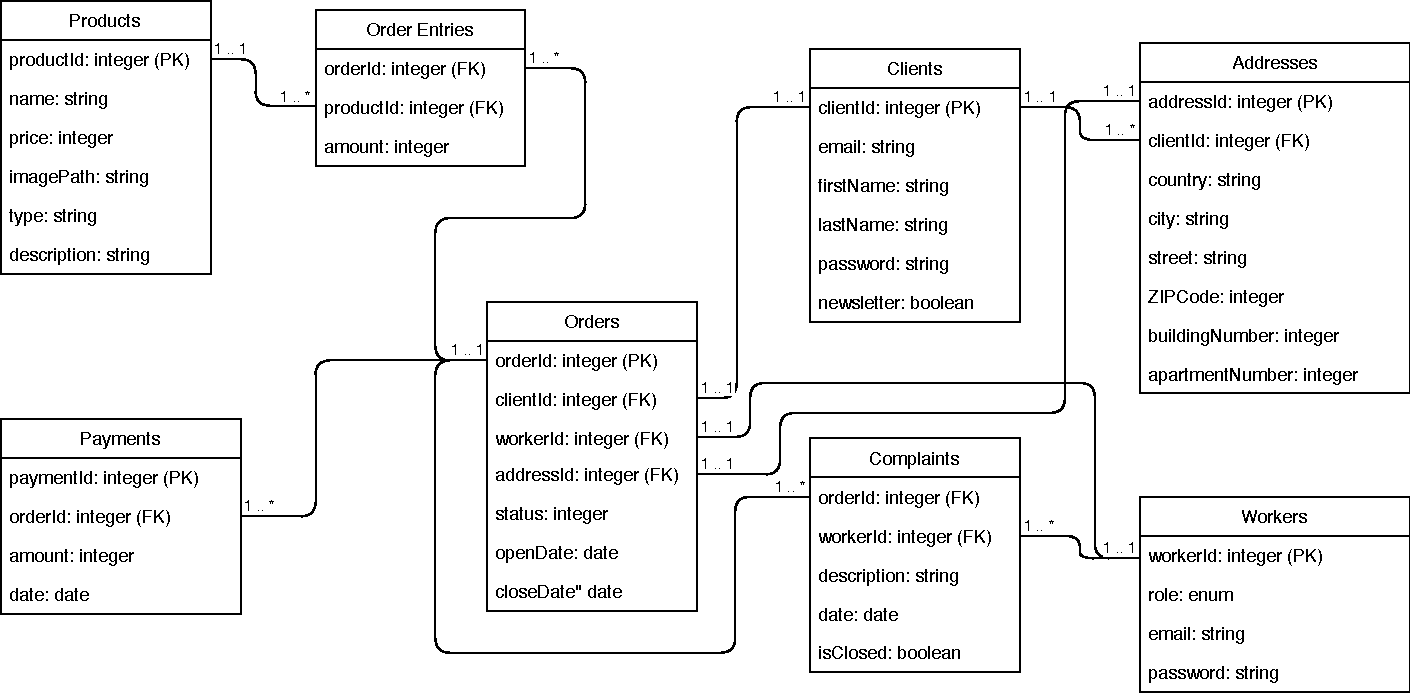
\includegraphics[width=500pt]{database.jpg}
	
	
%---------------------------------------	
	\chapter{Model dynamiki - diagramy STD}
	
%---------------------------------------	
	\chapter{Specyfikacja procesów PSPEC}
	
	
%---------------------------------------	
	\chapter{Słownik danych}
	
%---------------------------------------	
	\chapter{Technologie i narzędzia}	
		\section{Technologie}
		\begin{itemize}
			\item JavaScript
			\item SignalR
			\item React
			\item nUnit
			\item .NET
			\item JestTest
			\item CircleCI
		\end{itemize}
		
		\section{Narzędzia}
		\begin{itemize}
			\item Visual Studio Code
			\item Visual Studio Community
			\item Selenium
			\item Chromium
		\end{itemize}
	
\end{document}